%version 1.01, date 07/03/16, auteur Mathieu MEDICI, Julie PAIN

\documentclass[asi, sansVersion]{picInsa}

\usepackage{vocabulaireUnipik}

\begin{document}

\title{Description du Diagramme de classe}
\author{\Mathieu, \Julie}
\date{01/03/2016} 

\maketitle

\tableofcontents

\chapter{Diagramme de classe}

%% Inclure le  diagramme de classe
\begin{landscape}
\begin{figure}
	\centering
	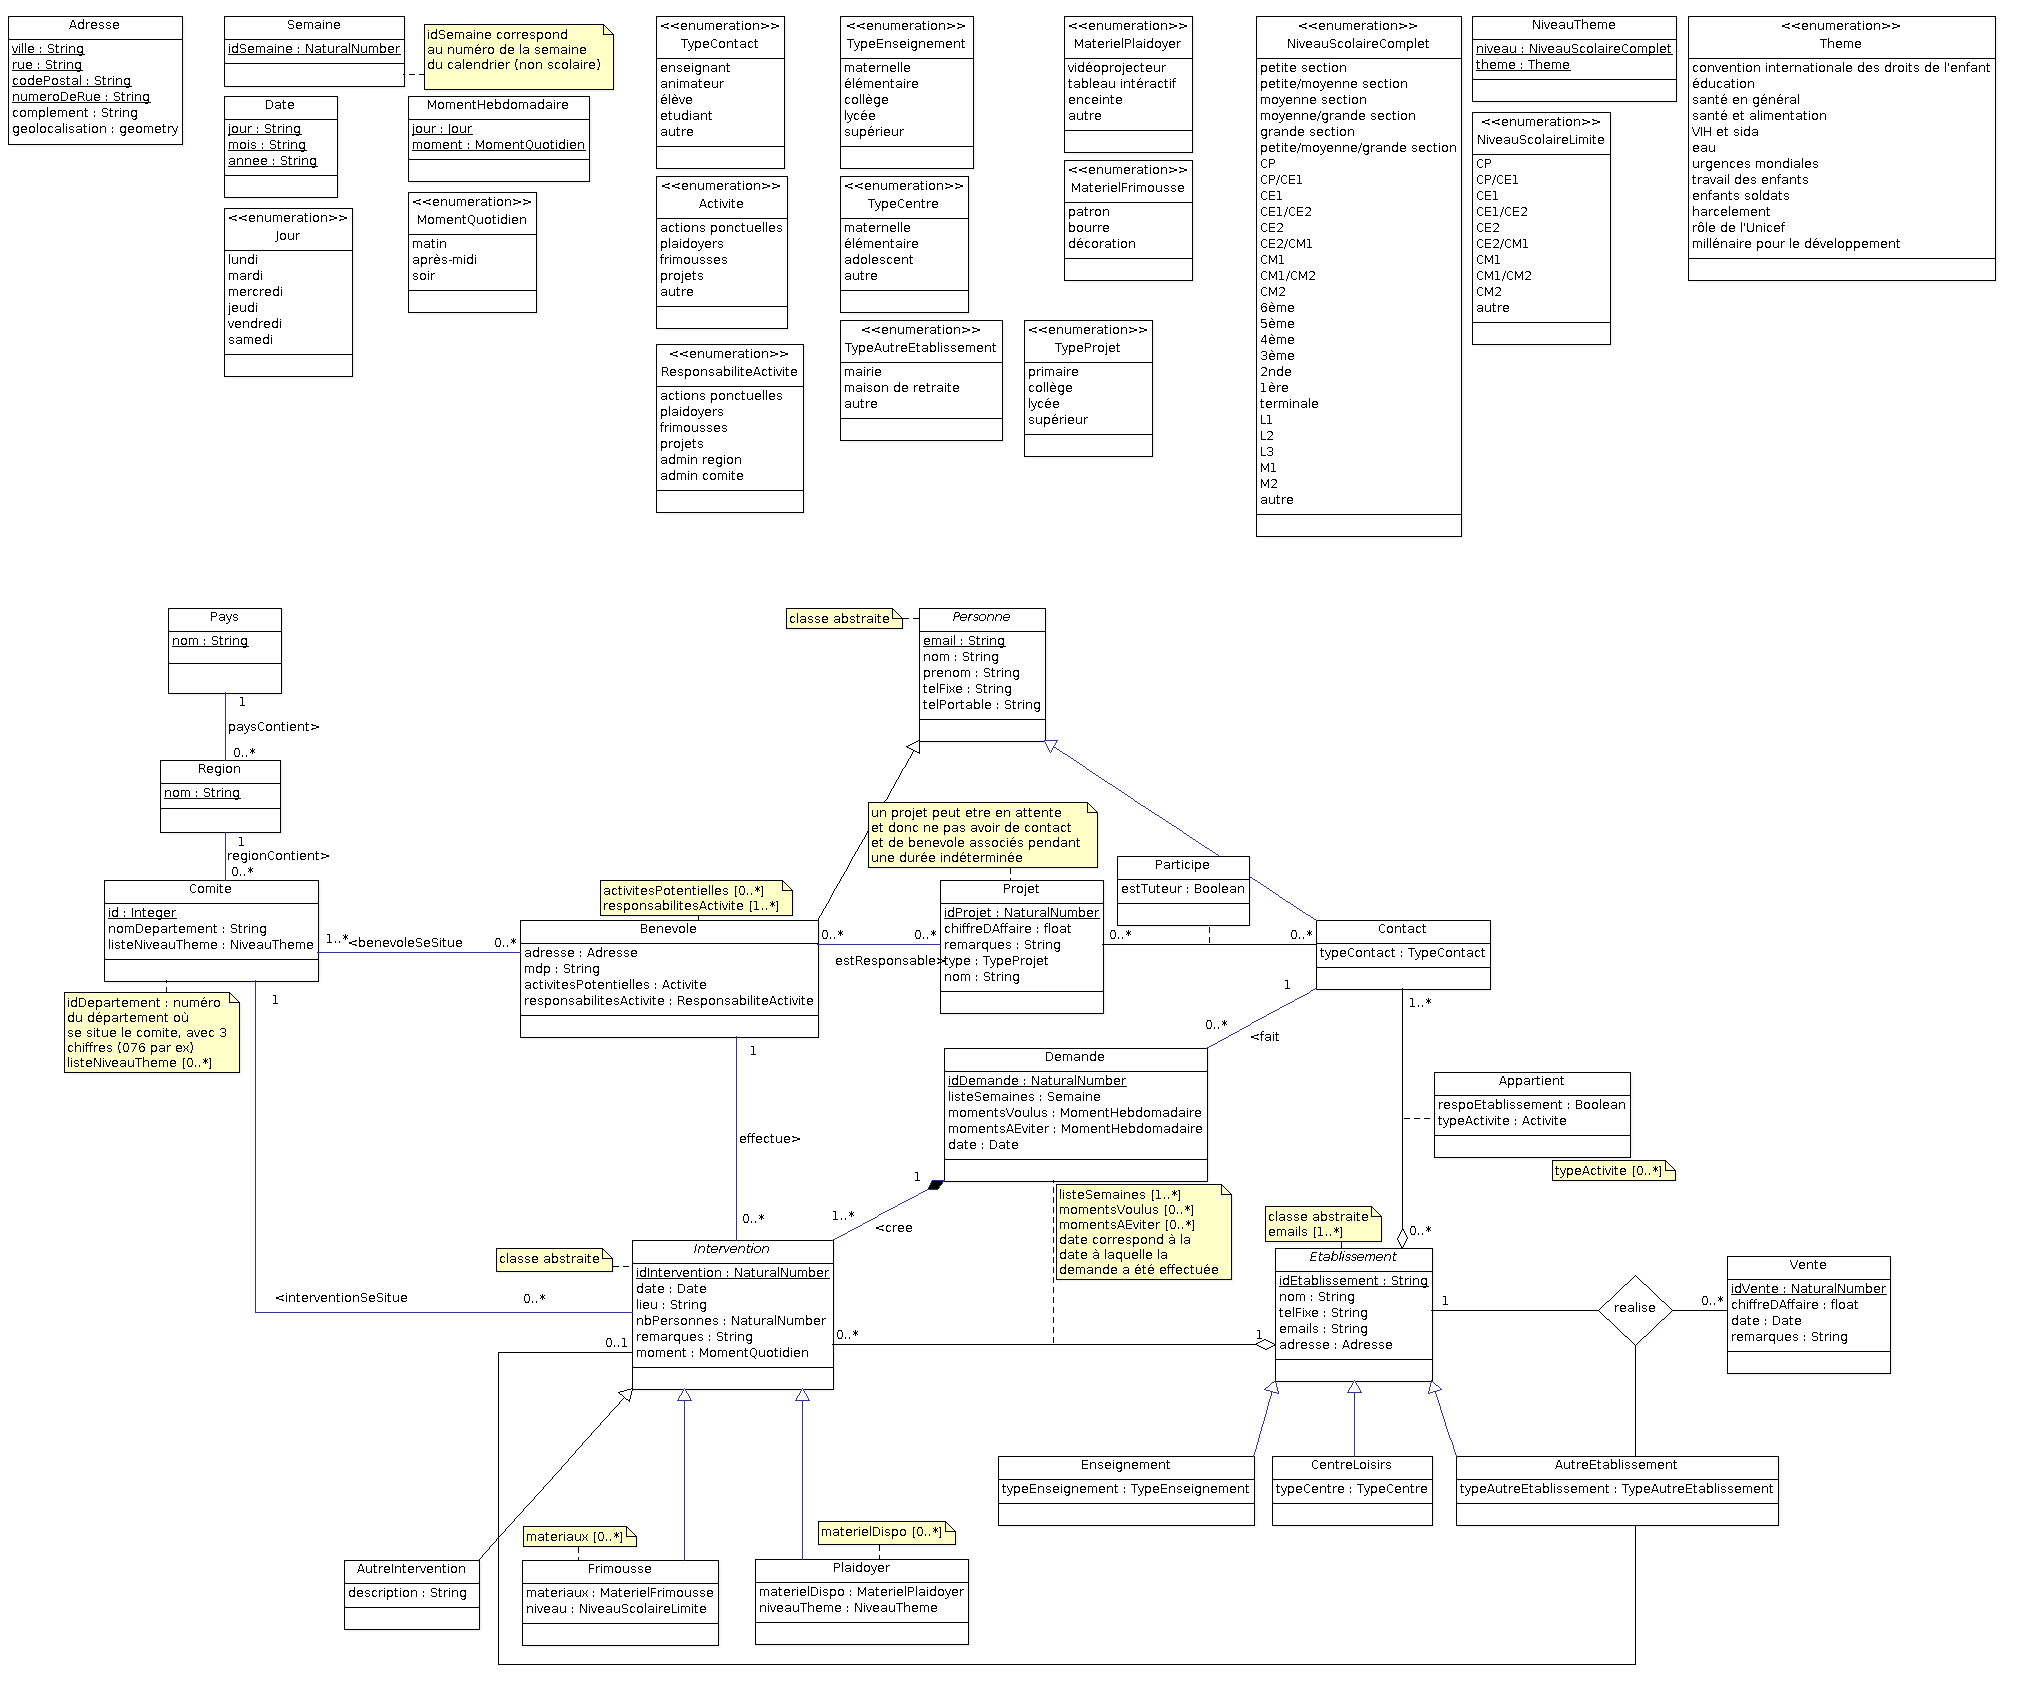
\includegraphics[scale=0.3]{images/diagrammeDeClasses}
	\caption{\label{modele}Diagramme de classe}
\end{figure}
\end{landscape}

\chapter{Description du Diagramme de classe}

Le diagramme de classe réalisé est composé de plusieurs types, de plusieurs classes et de plusieurs associations. Nous allons les décrire dans cette partie. \\ 

\section{Les types}

\subsection*{Geometry}

Le type geometry est un type de données respectant la norme de l'OGC (Open Geospatial Consortium) et qui définit la géolocalisation.

%\subsection*{Theme}

%Le type Theme est une énumération qui définit les différents thèmes possibles pour les plaidoyers.

\subsection*{NiveauScolaire}

Le type NiveauScolaire est une énumération qui définit tous les niveaux possibles pour les interventions. Ce type comporte aussi des combinaisons des niveaux comme par exemple "CPCE1" ou "CM1CM2". La valeur "autre" est utilisée pour des cas particuliers (niveau CLIS, CM26eme).

\subsection*{TypeCentre}

Le type TypeCentre est une énumération qui définit les différents niveaux pour les centres de loisirs.

\subsection*{TypeEnseignement}

Le type TypeEnseignement est une énumération qui définit les différents niveaux pour les enseignements.

\subsection*{TypeProjet}

Le type TypeProjet est une énumération qui définit les différents niveaux pour les projets.

\subsection*{TypeContact}

Le type TypeContact est une énumération qui définit les différents contacts possibles.

\subsection*{Materiel}

Le type Materiel est une énumération qui définit les différents types de matériel possibles pour les interventions plaidoyers.

\subsection*{MaterielFrimousse}

Le type MaterielFrimousse est une énumération qui définit les différents matériaux possibles pour les interventions frimousses.

\subsection*{Activite}

Le type Activite est une énumération qui définit les différentes activités que peuvent réaliser les bénévoles.

\subsection*{Jour}

Le type Jour est une énumération qui définit les différents jours possibles pour une intervention.

\subsection*{MomentQuotidien}

Le type MomentQuotidien est une énumération qui définit les différents moments possibles dans une journée, donc matin ou après-midi.

\subsection*{MomentHebdomadaire}

La classe MomentHebdomadaire définit un type qui est la combinaison d'un jour et d'un moment quotidien.\\
Cette classe a plusieurs attributs :
\begin{itemize}
\item un jour qui appartient à l'énumération Jour;
\item un moment qui appartient à l'énumération MomentQuotidien.
\end{itemize}

\subsection*{NiveauTheme}

La classe NiveauTheme définit un type qui est la combinaison d'un thème et d'un niveau.\\
Cette classe a plusieurs attributs : 
\begin{itemize}
\item un niveau qui appartient à l'énumération NiveauScolaire;
\item un thème.
\end{itemize}

\subsection*{Semaine}

La classe Semaine définit un type qui est une semaine du calendrier.\\
Cette classe a un attribut : 
\begin{itemize}
\item un identifiant unique.
\end{itemize}

\subsection*{Adresse}

La classe Adresse définit un type qui est l'adresse d'une personne ou d'un établissement.\\
Cette classe a plusieurs attributs : 
\begin{itemize}
\item une ville;
\item une rue;
\item un code postal;
\item un numéro de rue avec si besoin le supplément "bis", "ter" ou "quater";
\item un complément si besoin;
\item la géolocalisation associée à cette adresse.
\end{itemize}

\subsection*{Date}

La classe Date définit un type qui est une date.\\
Cette classe a plusieurs attributs : 
\begin{itemize}
\item un jour;
\item un mois;
\item une année.
\end{itemize}


\section{Les classes}

\subsection*{Personne}

La classe Personne est la classe mère des classes Benevole et Contact. C'est une généralisation, c'est à dire que la classe Personne est une classe abstraite et donc une Personne est soit un contact, soit un bénévole. \\
Cette classe a plusieurs attributs : 
\begin{itemize}
\item un nom;
\item un prénom;
\item un email;
\item un numéro de téléphone fixe;
\item un numéro de téléphone portable.
\end{itemize}

\subsection*{Benevole}

La classe Benevole est une classe fille de la classe Personne et la classe mère des classes AdminActivite, AdminComite et AdminRegion. Cette classe décrit les bénévoles de l'UNICEF qui réaliseront des interventions mais aussi ceux qui géreront des activités (AdminActivite), des comités (AdminComite) ou des régions (AdminRegion). L'héritage est ici une spécialisation, c'est à dire qu'une personne peut être simplement bénévole sans être administrateur. \\
Cette classe a plusieurs attributs : 
\begin{itemize}
\item une adresse correspondant à la rue, au numéro de rue, au code postal, à la ville, au complément si besoin et à une géolocalisation;
\item un mot de passe;
\item aucune, une ou plusieurs activités potentielles (action ponctuelle, frimousse, plaidoyer ou autre).
\end{itemize}

\subsection*{AdminActivite}

La classe AdminActivite permet de représenter un administrateur d'une ou plusieurs activités (administrateur local du cahier des charges). Cette classe est une classe fille de la classe Benevole.\\
Cette classe a un attribut :
\begin{itemize}
\item une ou plusieurs responsabilités d'activité (action ponctuelle, frimousse, plaidoyer ou autre). 
\end{itemize}

\subsection*{AdminComite}

La classe AdminComite permet de représenter un administrateur de comité (ou d'un département, c'est la même chose). Cette classe est une classe fille de la classe Benevole. 

\subsection*{AdminRegion}

La classe AdminRegion permet de représenter un administrateur de région, une région ayant en générale plusieurs comités. Cette classe est une classe fille de la classe Benevole. 

\subsection*{Contact}

La classe Contact est une classe fille de la classe Personne. Cette classe décrit les personnes étant reliées à un établissement comme le personnel y travaillant ou encore les élèves. \\
Cette classe a un attribut : 
\begin{itemize}
\item un type de contact qui permet de déterminer si un contact est un enseignant, un animateur, un élève ou autre.
\end{itemize} 


\subsection*{Etablissement}

La classe Etablissement est la classe mère des classes Enseignement et CentreLoisirs. C'est une spécialisation, c'est à dire qu'un établissement peut être ni un enseignement ni un centre de loisirs. Ce sera le cas pour les mairies par exemple. \\
Cette classe a plusieurs attributs : 
\begin{itemize}
\item un identifiant unique;
\item un nom;
\item un numéro de téléphone fixe;
\item une ou plusieurs adresses e-mail;
\item une adresse correspondant à la rue, au numéro de rue, au code postal, à la ville, au complément si besoin et à une géolocalisation.
\end{itemize}

\subsection*{Enseignement}
La classe Enseignement est une classe fille de la classe Etablissement. Cette classe décrit les établissements qui relèvent de l'Education Nationale. \\
Cette classe a plusieurs attributs : 
\begin{itemize}
\item un UAI (Unité Administrative Immatriculée) qui est une combinaison de chiffres et de lettres unique pour chaque enseignement;
\item un type d'enseignement qui permet de déterminer si l'enseignement est une école maternelle, une école élémentaire, un collège, un lycée ou un établissement supérieur. 
\end{itemize} 


\subsection*{CentreLoisirs}
La classe CentreLoisirs est une classe fille de la classe Etablissement. Cette classe décrit les établissements ayant un rapport avec les loisirs. \\
Cette classe a un attribut : 
\begin{itemize}
\item un type de centre de loisirs qui permet de déterminer si un centre de loisirs prend en charge des enfants d'école maternelle, d'école élémentaire ou des adolescents.
\end{itemize}  

\subsection*{Intervention}
La classe Intervention est la classe mère des classes Plaidoyer et Frimousse. Cette classe décrit une intervention que peut demander un contact. \\
Cette classe a plusieurs attributs :
\begin{itemize}
\item une date précise déterminée par les bénévoles lors de l'attribution des bénévoles aux interventions;
\item un identifiant unique;
\item un lieu dans l'établissement, c'est à dire la salle où aura lieu l'intervention;
\item le nombre de personnes concernées par cette intervention (exemple : le nombre d'élève d'une classe);
\item un champ remarque permettant au contact de saisir des remarques spécifiques à cette intervention;
\item un moment indiquant si l'intervention a lieu le matin, l'après-midi ou les deux.
\end{itemize}

\subsection*{Plaidoyer}
La classe Plaidoyer est une classe fille de la classe Intervention. \\
Cette classe a un attribut : 
\begin{itemize}
\item le matériel disponible pour l'intervention (présence ou non d'un vidéoprojecteur, d'un tableau intéractif, d'enceintes ou autre).
\end{itemize}

\subsection*{Frimousse}
La classe Frimousse est une classe fille de la classe Intervention. Une activité frimousse est réalisée avec des enfants d'école élémentaire. \\
Cette classe a un attribut :
\begin{itemize}
\item les matériaux nécessaires à la réalisation de l'activité (patron, bourre, décoration).
\end{itemize}

\subsection*{Projet}
La classe Projet représente les projets réalisées par des étudiants ou des lycéens.\\
Cette classe a plusieurs attributs : 
\begin{itemize}
\item un identifiant unique;
\item le chiffre d'affaire réalisés par ce projet;\item la description du projet est un champ permettant au(x) bénévole(s) de saisir d'autres informations importantes sur le projet (nom du projet par exemple);
\item le type de projet permet de savoir si le projet est réalisé par des étudiants, des lycéens, des élèves d'école primaire ou de collège.
\end{itemize}

\subsection*{Vente}
La classe Vente représente les actions ponctuelles réalisées par les établissements.\\ 
Cette classe a plusieurs attributs : 
\begin{itemize}
\item un identifiant unique; 
\item le chiffre d'affaire réalisé par cette vente;
\item la date de la vente;
\item un champ remarques permettant aux bénévoles d'ajouter des informations importantes. 
\end{itemize}

\subsection*{Demande}

La classe Demande représente les demandes d'intervention effectuées par les contacts.\\
Cette classe a plusieurs attributs :
\begin{itemize}
\item un identifiant unique; 
\item une liste des semaines correspondant aux semaines où le contact est disponible; 
\item les moments voulus pour une semaine type (sera donc valable pour toutes les semaines où le contact est disponible);
\item les moments à éviter pour une semaine type. 
\end{itemize}

\subsection*{Comite}

La classe Comite représente les comités de bénévoles, il y a un comité par département.\\
Cette classe a plusieurs attributs :
\begin{itemize}
\item un identifiant unique (le numéro du département sous la forme XXX);
\item le nom du département;
\item la liste des thèmes du comité avec les niveaux associés à chaque thème.
\end{itemize}

\subsection*{Region}

La classe Region représente les régions françaises.\\
Cette classe a un attribut :
\begin{itemize}
\item le nom de la région.
\end{itemize}

\subsection*{Pays}

La classe Pays représente la France.\\
Cette classe a un attribut :
\begin{itemize}
\item le nom du pays (donc "France").
\end{itemize}


\section{Les associations}

\subsection*{estResponsable}
L'association \textit{estResponsable} relie un Benevole et un Projet. Un benévole est responsable d'aucun, un ou plusieurs projets et un projet est sous la responsabilité d'aucun (si le projet est en attente), un ou plusieurs bénévoles.

\subsection*{Participe}
L'association \textit{Participe} relie un Contact et un Projet. Un contact participe à aucun, un ou plusieurs projets et un projet a pour participant aucun (si le projet est en attente), un ou plusieurs contacts.\\
Cette association a un attribut :
\begin{itemize}
\item un booléen qui indique si le contact est ou non un tuteur du projet (un professeur tuteur des élèves réalisant le projet par exemple). 
\end{itemize}

\subsection*{realise}

L'association \textit{realise} est une association ternaire qui relie une Vente, un Etablissement et une Intervention. Un établissement réalise aucune, une ou plusieurs ventes. Une vente est réalisée par un et un seul établissement. La vente a été réalisée suite à aucune ou une intervention.

\subsection*{fait}

L'association \textit{fait} relie un Contact et une Demande. Un contact fait aucune, une ou plusieurs demandes, une demande est faite par un et un seul contact.

\subsection*{cree}

L'association \textit{cree} relie une Demande et une Intervention. Une demande crée une ou plusieurs interventions, une intervention est créée par une et une seule demande.

\subsection*{effectue} 

L'association \textit{effectue} relie un Benevole et une Intervention. Un bénévole effectue aucune, une ou plusieurs interventions. Une intervention est effectuée par un et un seul bénévole. 

\subsection*{Appartient}

L'association \textit{Appartient} relie un Contact et un Etablissement. Un contact appartient à aucun, un ou plusieurs établissements. Un établissement a un ou plusieurs contacts.\\
Cette association a plusieurs attributs :
\begin{itemize}
\item un booléen qui indique si le contact est ou non le responsable de l'établissement; 
\item un type qui indique quelles sont les responsabilités du contact par rapport aux activités.
\end{itemize}

\subsection*{effectuerDans}

L'association \textit{estEffectueDans} relie une Intervention et un Etablissement. Une intervention est effectuée dans un et un seul établissement, un établissement peut être le lieu d'aucune, une ou plusieurs interventions.

\subsection*{benevoleSeSitue}

L'association \textit{benevoleSeSitue} relie un Benevole et un Departement. Un bénévole se situe dans un et un seul département, un département a aucun, un ou plusieurs bénévoles.

\subsection*{interventionSeSitue}

L'association \textit{interventionSeSitue} relie une Intervention et un Departement. Une intervention se situe dans un et un seul département, un département a aucune, une ou plusieurs interventions.

\subsection*{regionContient}

L'association \textit{regionContient} relie une Region et un Comite. Une région contient aucun, un ou plusieurs comités, un comité est dans une et une seule région.

\subsection*{paysContient}

L'association \textit{paysContient} relie un Pays et une Region. Un pays contient aucune, une ou plusieurs régions, une région est dans un et un seul pays.

\chapter{Contraites d'intégrité}

\section{Les contraintes d'intégrité intra-classe}
Dans cette partie, nous allons décrire les différentes contraintes d'intégrité de chaque classe et classe-association.
 
\subsection*{Personne}
Contraintes de domaine et de nullité des attributs :
\begin{itemize}
 	\item \textbf{nom :} chaine de caractère de longueur de 100 caractères au maximum, attribut non nul;
	\item \textbf{prénom :} chaine de caractère de longueur de 100 caractères au maximum, attribut non nul;
	\item \textbf{email :} chaine de caractère de longueur de 100 caractères au maximum, la syntaxe de l'e-mail doit être la suivante : user@host.domain\\
	user : contient des chiffres/lettres ainsi que les symboles "\_", "-", "." \\
	host : contient des chiffres/lettres \\
	domain : chaine de caractère composée de 2 ou 3 lettres. \\
	attribut non nul;  
	\item \textbf{telFixe :} chaine de caractère composée de 10 chiffres commençant par "0", attribut peut être nul;
	\item \textbf{telPortable :} chaine de caractère composée de 10 chiffres commençant par "0", attribut peut être nul.\\
\end{itemize}  

\subsection*{Benevole}
Contraintes de domaine et de nullité des attributs :
\begin{itemize}
 	\item \textbf{adresse :} constante de type \textbf{Adresse}, attribut non nul;
	\item \textbf{mdp :} chaine de caractère de longueur de 50 caractères au maximum, de 8 caractères au minimum, attribut non nul;  
	\item \textbf{activitesPotentielles :} constante de type \textbf{Activite}, atrribut multivalué, peut être nul.\\
\end{itemize}  

\subsection*{AdminLocal}
Contraintes de domaine et de nullité des attributs :\\
 \indent \indent \textbf{responsabiliteActivite :} constante de type \textbf{Activite}, attribut multivalué, peut être nul.\\

 
\subsection*{Contact}
Contraintes de domaine et de nullité des attributs :\\
\indent \indent \textbf{type :} constante de type \textbf{TypeContact},attribut non nul.\\

\subsection*{Etablissement}
Contraintes de domaine et de nullité des attributs :
\begin{itemize}
 	\item \textbf{idEtablissement :} chaine de caractère de longueur de 100 caractères au maximum, attribut non nul;
	\item \textbf{nom :} chaine de caractère de longueur de 100 caractères au maximum, attribut non nul;
	\item \textbf{telFixe :} chaine de caractère composée de 10 chiffres commençant par "0", attribut peut être nul;
	\item \textbf{email :} chaine de caractère de longueur de 100 caractères au maximum, la syntaxe de l'e-mail doit être la suivante : user@host.domain\\
	user : contient des chiffres/lettres ainsi que les symboles "\_", "-", "." \\
	host : contient des chiffres/lettres \\
	domain : chaine de caractère composée de 2 ou 3 lettres. \\
	attribut multivalué, non nul; 
	\item \textbf{adresse :} constante de type \textbf{Adresse}, attribut non nul; 
	\item \textbf{geolocalisation :} constante de type \textbf{geometry}, attribut non nul.\\
\end{itemize}  

\subsection*{Enseignement}
Contraintes de domaine et de nullité des attributs :
\begin{itemize}
	\item \textbf{UAI :} chaine de caractères composée de lettre et de chiffres, attribut non nul;
	\item \textbf{type :} constante de type \textbf{TypeEnseignement}, attribut non nul.\\
\end{itemize}

\subsection*{CentreLoisirs}
Contraintes de domaine et de nullité des attributs :\\
\indent \indent \textbf{type :} constante de type \textbf{TypeCentre}, peut être nul.\\

\subsection*{Intervention} 
Contraintes de domaine et de nullité des attributs :
\begin{itemize}
 	\item \textbf{idIntervention :} entier, attribut non nul;
	\item \textbf{date :} chaine de caractère de longueur de 10 caractères ayant la syntaxe suivante "JJ/MM/AAAA", attribut non nul;
	\item \textbf{lieu :} chaine de caractère composée de chiffres et de lettres, attribut peut être nul;
	\item \textbf{nbPersonnes :} entier, attribut non nul;  
	\item \textbf{materielDispo :} constante de type \textbf{Matériel}, attribut multivalué non nul; 
	\item \textbf{remarques :} chaine de caractères de longueur de 1000 caractères au maximum;
	\item \textbf{moment :} constante de type \textbf{MomentJournalier}, attribut peut être nul;\\
\end{itemize}  

\subsection*{Plaidoyer}
Contraintes de domaine et de nullité des attributs :\\
\indent \indent \textbf{niveauThème :} constante de type \textbf{niveauThème}, attribut non nul.\\

\subsection*{Frimousse}
Contraintes de domaine et de nullité des attributs :
\begin{itemize}
	\item \textbf{materiaux :} constante de type \textbf{MaterielFrimousse}, attribut multivalué non nul;
	\item \textbf{niveaux :} constante de type \textbf{NiveauScolaireLimite}, attribut non nul.\\
\end{itemize}

\subsection*{Projet}
Contraintes de domaine et de nullité des attributs :
\begin{itemize}
 	\item \textbf{idProjet :} entier, attribut non nul;
	\item \textbf{chiffreDAffaire :} Entier, attribut non nul;
	\item \textbf{description :} chaine de caractère composée de longueur de 1000 caractères au maximum, attribut ne peut être nul;
	\item \textbf{type :} constante de type \textbf{TypeProjet}, attribut non nul. \\  
\end{itemize} 

\subsection*{Vente}
Contraintes de domaine et de nullité des attributs :
\begin{itemize}
 	\item \textbf{idVente :} entier, attribut non nul;
	\item \textbf{chiffreDAffaire :} Entier, attribut non nul;
	\item \textbf{date :} chaine de caractère de longueur de 10 caractères ayant la syntaxe suivante "JJ/MM/AAAA", attribut non nul;
	\item \textbf{remarques :} chaine de caractères de longueur de 1000 caractères au maximum. \\  
\end{itemize} 

\subsection*{Demande}
Contraintes de domaine et de nullité des attributs :
\begin{itemize}
 	\item \textbf{idDemande :} entier, attribut non nul;
	\item \textbf{momentsVoulus :} constante de type \textbf{MomentHebdomadaire}, attribut multivalué non nul;
	\item \textbf{momentsVoulus :} constante de type \textbf{MomentHebdomadaire}, attribut multivalué non nul;
	\item \textbf{date :} chaine de caractère de longueur de 10 caractères ayant la syntaxe suivante "JJ/MM/AAAA", attribut non nul. \\
\end{itemize} 

\subsection*{Departement}
Contraintes de domaine et de nullité des attributs :
\begin{itemize}
	\item \textbf{idDepartement :} Entier, attribut non nul;
	\item \textbf{nom :} chaine de caractère de longueur de 100 caractères au maximum, attribut non nul.\\
\end{itemize}

\subsection*{Adresse}
Contraintes de domaine et de nullité des attributs :
\begin{itemize}
 	\item \textbf{ville :} chaine de caractère de longueur de 100 caractères au maximum, attribut non nul;
	\item \textbf{rue :} chaine de caractère de longueur de 500 caractères au maximum, attribut non nul;
	\item \textbf{numeroDeRue :} chaine de caractère composée d'un numéro et, si besoin, de "bis", "ter", "quater", attribut non nul; 
	\item \textbf{complement : } chaine de caractère de longueur de 100 caractères au maximum;
	\item \textbf{codePostale :} chaine de caractère composée de 5 chiffres, attribut non nul.\\
\end{itemize}

\subsection*{NiveauTheme}
Contraintes de domaine et de nullité des attributs :
\begin{itemize}
	\item \textbf{niveau :} constante de type \textbf{NiveauScolaireComplet}, attribut non nul;
	\item \textbf{theme :} constante de type \textbf{Theme}, attribut non nul.\\
\end{itemize}

Autres contraintes :

Si le niveau est "petiteSection", "petiteMoyenneSection", "moyenneSection", "moyenneGrandeSection", "grandeSection", ou "petiteMoyenneGrandeSection", le thème associé doit être un des thèmes suivants : "conventionInternationaleDesDroitsDeLEnfant", "education", "laSanteAlimentation", "eau" et "harcelement". 

Si le niveau est "CP", "CPCE1", "CE1", "CE1CE2", "CE2", "CE2CM1", "CM1", "CM1CM2" ou "CM2", le thème associé doit être un des thèmes suivants : "conventionInternationaleDesDroitsDeLEnfant", "education", "laSanteEnGeneral", "santeAlimentation", "eau", "travailDesEnfants" et "harcelement".

Si le niveau est "6eme", "5eme", "4eme" ou "3eme", le thème associé doit être un des thèmes suivants : "conventionInternationaleDesDroitsDeLEnfant", "education", "laSanteEnGeneral", "santeAlimentation", "eau", "urgencesMondiales", "travailDesEnfants", "enfantsSoldats" et "harcelement".

Si le niveau est "2nde", "1ere", "terminale", "L1", "L2", "L3", "M1", "M2" ou "autre" le thème associé doit être un des thèmes suivants : "conventionInternationaleDesDroitsDeLEnfant", "education", "laSanteEnGeneral", "santeAlimentation", "vihSida", "eau", "urgencesMondiales", "travailDesEnfants", "enfantsSoldats", "harcelement", "roleDeLUnicef" et "millenairePourLeDeveloppement".\\

\subsection*{Participe}
Contraintes de domaine et de nullité des attributs :\\
\indent \indent \textbf{estTuteur :} Booléen, attribut non nul.\\


\subsection*{Appartient}
Contraintes de domaine et de nullité des attributs :
\begin{itemize}
	\item \textbf{respoEtablissement :} , attribut non nul;
	\item \textbf{type :} constante de type \textbf{Activite}, attribut multivalué peut être nul.
\end{itemize}

\section{Les contraintes d'intégrités inter-classe}

\subsection*{Etablissement - Enseignement}
L'\textbf{idEtablissement} d'un établissement doit correspondre à l'\textbf{UAI} si cette établissement est une instance d'enseignement.\\

\subsection*{Intervention - Plaidoyer}
Le \textbf{niveau} d'une intervention frimousse ainsi que le \textbf{niveau} (de NiveauTheme) d'une intervention plaidoyer doit être en correspondance avec le \textbf{type} de l'établissement.  

Si l'établissement est un enseignement, le \textbf{niveau} peut prendre différentes valeurs selon le \textbf{type}:
\begin{itemize}
\item Si le \textbf{type} est "maternelle", le \textbf{niveau} peut être : "petiteSection", "petiteMoyenneSection", "moyenneSection", "moyenneGrandeSection", "grandeSection", "petiteMoyenneGrandeSection" ou "autre";
\item Si le \textbf{type} est "elementaire", le \textbf{niveau} peut être : "CP", "CPCE1", "CE1", "CE1CE2", "CE2", "CE2CM1", "CM1", "CM1CM2", "CM2" ou "autre";
\item Si le \textbf{type} est "college", le \textbf{niveau} peut être : "6eme", "5eme", "4eme", "3eme" ou "autre";
\item Si le \textbf{type} est "lycee", le \textbf{niveau} peut être : "2nde", "1ere", "terminale" ou "autre";
\item Si le \textbf{type} est "superieur", le \textbf{niveau} peut être : "L1", "L2", "L3", "M1", "M2" ou "autre".
\end{itemize}

Si l'établissement est un centre de loisirs, le \textbf{niveau} peut prendre différentes valeurs selon le \textbf{type}:
\begin{itemize}
\item Si le \textbf{type} est "maternelle", le \textbf{niveau} peut être : "petiteSection", "petiteMoyenneSection", "moyenneSection", "moyenneGrandeSection", "grandeSection", "petiteMoyenneGrandeSection" ou "autre";
\item Si le \textbf{type} est "elementaire", le \textbf{niveau} peut être : "CP", "CPCE1", "CE1", "CE1CE2", "CE2", "CE2CM1", "CM1", "CM1CM2", "CM2" ou "autre";
\item Si le \textbf{type} est "adolescent", le \textbf{niveau} peut être : "6eme", "5eme", "4eme", "3eme", "2nde", "1ere", "terminale" ou "autre". 
\end{itemize}

\chapter{Les dépendances fonctionnelles}

Dans cette partie, nous allons déterminer les dépendances fonctionnelles de chaque classe. \\ 

\subsection*{Personne}
\begin{itemize}
\item[] email $\rightarrow$ nom 
\item[] email $\rightarrow$ prenom 
\item[] email $\rightarrow$ telFixe 
\item[] email $\rightarrow$ telPortable 
\item[] telPortable $\rightarrow$ nom
\item[] telPortable $\rightarrow$ prenom
\item[] telFixe $\rightarrow$ nom
\end{itemize}


\subsection*{Contact}
\begin{itemize}
\item[] email $\rightarrow$ type 
\end{itemize}

\subsection*{Benevole}
\begin{itemize}
\item[] email $\rightarrow$ adresse 
\item[] email $\rightarrow$ mdp 
\item[] email $\rightarrow$ activitesPotentielles 
\end{itemize}


\subsection*{AdminLocal}
\begin{itemize}
\item[]email $\rightarrow$ activitesPotentielles 
\end{itemize}

\subsection*{Etablissement}
\begin{itemize}
\item[] idEtablissement $\rightarrow$ nom 
\item[] idEtablissement $\rightarrow$ telFixe
\item[] idEtablissement $\rightarrow$ email
\item[] idEtablissement $\rightarrow$ adresse
\item[] idEtablissement $\rightarrow$ geolocalisation
\item[] geolocalisation $\rightarrow$ adresse
\item[] telFixe $\rightarrow$ nom
\item[] adresse $\rightarrow$ nom
\end{itemize}

\subsection*{CentreLoisirs}
\begin{itemize}
\item[]	idEtablissement $\rightarrow$ type
\end{itemize}

\subsection*{Enseignement}
\begin{itemize}
\item[]	idEtablissement $\rightarrow$ type
\item[] idEtablissement $\rightarrow$ UAI
\item[] UAI $\rightarrow$ type
\end{itemize}

\subsection*{Intervention}
\begin{itemize}
\item[]	idIntervention $\rightarrow$ date
\item[]	idIntervention $\rightarrow$ lieu
\item[]	idIntervention $\rightarrow$ nbPersonnes
\item[]	idIntervention $\rightarrow$ materielDispo
\item[]	idIntervention $\rightarrow$ remarques
\item[]	idIntervention $\rightarrow$ moment
\end{itemize}

\subsection*{Plaidoyer}
\begin{itemize}
\item[]	idIntervention $\rightarrow$ niveauTheme
\end{itemize}

\subsection*{Frimousse}
\begin{itemize}
\item[]	idIntervention $\rightarrow$ materiaux
\item[] idIntervention $\rightarrow$ niveau
\end{itemize}

\subsection*{Projet}
\begin{itemize}
\item[] idProjet $\rightarrow$ chiffreDaffaire
\item[] idProjet $\rightarrow$ description
\item[] idProjet $\rightarrow$ type
\end{itemize}

\subsection*{Vente}
\begin{itemize}
\item[]	idVente $\rightarrow$ chiffreDaffaire
\item[]	idVente $\rightarrow$ date
\item[]	idVente $\rightarrow$ remarques
\end{itemize}

\subsection*{Departement}
\begin{itemize}
\item[] idDepartement $\rightarrow$ nom
\end{itemize}

\subsection*{Demande}
\begin{itemize}
\item[] idDemande $\rightarrow$ listeDemaines 
\item[] idDemande $\rightarrow$ momentsVoulus
\item[] idDemande $\rightarrow$ momentsAEviter
\end{itemize}
 



\end{document}
